


\pagebreak 
\section{Consumption Analysis}
%\subsection{Calibration Review}
%\subsection{Partial Equilibrium Comparison}
Since the primary novelty of HANKs models compared with simpler NK models lie in the consumption/savings dynamics it stands to reason to review these dynamics, and discuss their empirical relevance and counterparts in other in models. First, I focus on the response of consumption to transitory shocks to income and the real interest rate, since these are the main drivers of consumption over the cycle. The second part discusses the implications for consumption responses of adding heterogeneity, and shows how a simple decomposition can split the aggregate HANK response into the response from a TANK model and a part relating to distributional dynamics. The remaining section conducts and discusses robustness w.r.t central parameters. 


%The left panel of figure \ref{fig:SS_dists} plots the estimated distribution of discount factors, while the right panel plots the marginal propensity to consume following a transitory income shock as a function of wealth. The aggregate MPC is 0.6 in period 1, which is in the middle of empirical estimates (\citet{souleles1999response}, \citet{shapiro2003consumer}, \citet{johnson2006household}, \citet{shapiro2009did}, \citet{sahm2010household}, \citet{broda2014economic}). As per the figure, the aggregate MPC is primarily driven by low wealth household, and in particular, the financially constrained who averages an MPC of 1.   \\
%Table \ref{table:Household_dist_stat} displays a number of statistics across different types of households. As also evident from the figure the MPC is largely depend on wealth, and to a much lesser extend income. 

%\subsubsection{The Marginal Propensity to Consume}
\subsection{Income shocks and Marginal Propensities to Consume}
To evaluate how well the calibrated model fit empirical consumption responses, I consider an experiment where households are subject to a transitory income shock where all households receive a lumpsum transfer corresponding to 1\% of the steady-state wage. The shock lasts only for one period, so as to match the shock carried out in \citet{auclert2018intertemporal}, since this allows for a comparison with empirical estimates of dynamic consumption responses. Figure \ref{fig:MPC_evidence_compare} plots the annual marginal propensity to consume following the shock along with the empirical estimates from \citet{fagereng2019mpc}. The authors here use lottery prizes in Norway as proxies for transitory income shocks to estimate the dynamic consumption response for households. The model fail to match the high initial MPC, but the persistence afterwards is reasonably well captured. A contemporaneous, annual MPC of 0.25 out of transitory income is not entirely consistent with the Norwegian evidence, but matches well other empirical estimates in the literature (\citet{souleles1999response}, \citet{shapiro2003consumer}, \citet{johnson2006household}, \citet{shapiro2009did}, \citet{sahm2010household}, \citet{broda2014economic} to name but a few).

The second panel (\ref{fig:MPC_wealth_SS}) plots the consumption functions for different values of $\beta$ along with the distribution of net worth. The figure partially reveals the effect of discount factors on MPCs (the slope of the consumption function), especially when taking into consideration the correlation between $\beta$ and wealth. For the most impatient the consumption function is steep, reflecting a high MPC. Since this type of household tends to be in the range with low net worth this further boosts the aggregate MPC. The slope of the consumption function for the most impatient is relatively more steep than in \citet{carroll2017distribution}, which is due to the low value of $\beta$ I obtain for these (0.913 vs 0.9867 in Carrol et. al).\footnote{Note though they assume a uniform distribution over discount factors, which I do not necessarily. The share of population on the lowest discount factors are 7\% vs. 17\% for my and Carrol et. al's calibrations respectively.  } 


%A low contemporaneous MPC is a well known weakness for the class of models in which heterogeneous-discount-factor HANK model belongs. For instance, \citet{hagedorn2019fiscal} construct a similar HANK model (minus the search-and-matching labor market) and, conditonal on calibration, obtains a quarterly MPC of 0.12 to a similar shock. For comparison, the quarterly MPC in my model is 0.19. \citet{auclert2018intertemporal} finds that a two asset HANK model a la \citet{kaplan2014model} or having bonds in the utility function as in \citet{kaplan2018microeconomic}, \citet{michaillat2018new}, \citet{hagedorn2018prices} is necessary to match the high initial MPCs. 

%The effect of bonds in the utility function is that it increases the savings stock, hence decreasing consumption for a given income. This in turn increases the marginal utility of consumption, and hence provides higher MPCs. However, since the HANK model in this paper is already calibrated to the wealth distribution in the data, this channel serves no purpose. Thus the solution would be to expand the model to contain both liquid and illiquid assets, but given the increased complexity of the model and the higher computational cost in the household's dynamic programming problem I opt to keep the more simple setup described above.  




\begin{figure}[H]
\makebox[\linewidth][c]{%
\centering
\begin{subfigure}{.5\textwidth}
  \centering
  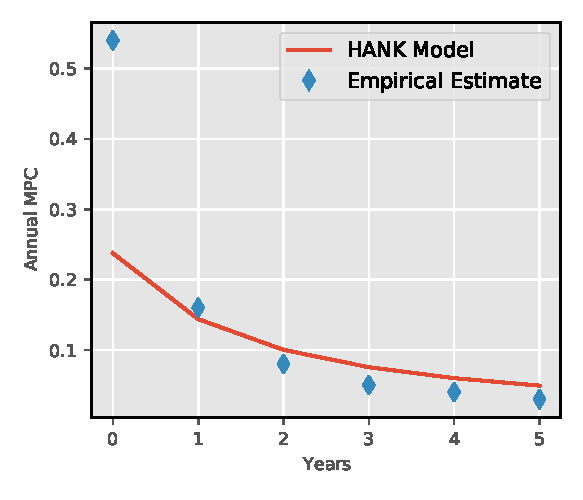
\includegraphics[width=.99\linewidth]{mainmatter/plots/SS_evaluation/Mpc_compare_Norway.pdf}
  \caption{Annual model MPCs vs. data. } \label{fig:MPC_evidence_compare}
\end{subfigure}%
\begin{subfigure}{.5\textwidth}
  \centering
  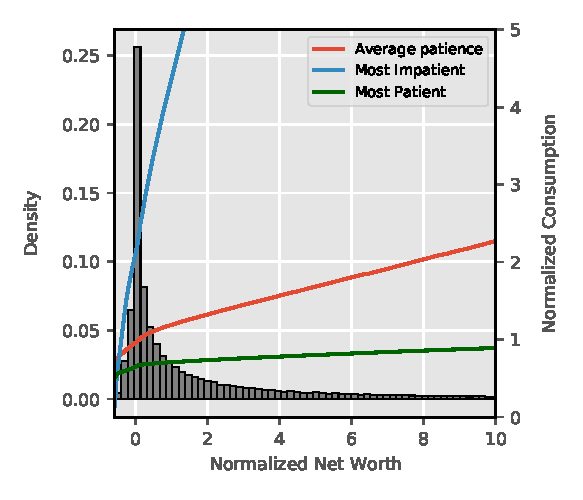
\includegraphics[width=.99\linewidth]{mainmatter/plots/SS_evaluation/Consumption_function.pdf}
  \caption{Consumption Functions and the distribution of Net worth. } \label{fig:MPC_wealth_SS}
\end{subfigure}
}
\caption[Caption for LOF]{Consumption Behavior}
\label{fig:SS_dists}
  {\scriptsize  a) Annual MPCs (calculated as $\sum_{t=0}^{3}\text{\ensuremath{\text{Quarterly MPC}_{t}}}=\sum_{t=0}^{3}\frac{dC_{t}}{dI_{t_{0}}}$) in the calibrated HANK model versus evidence from \citet{fagereng2019mpc} b) Consumption function for consumers with lowest, average and highest $\beta$ respectively and histogram of cash on hand $m_{ss}= a_{ss} + (1+\tau^{VAT}) c_{ss}$. In panel (b), all variables are normalised by income. }
\end{figure}


\subsection{Consumption and Interest rates}
I review the interest rate response for two reasons: 1) The sensitivity of consumption to interest rates vs income is obviously a key determinant in the cyclical response of consumption, 2) Determinacy. Regarding the second point recall that in the canonical NK model a sufficient condition for determinacy is that the Taylor principle is satisfied (nominal interest rate responds more than one-to-one to inflation). This applies since an increase in the real interest rate decrease consumption in the present periods thereby lowering aggregate demand and hence inflation. Since HANK models feature a generally weaker interest rate response, determinacy might not be obtained as easily.  
%This is not necessarily the case in HANK models, see for instance the results in \citet{ravn2016macroeconomic}, \citet{acharya2020understanding}. 


Figure \ref{fig:calibration_C_r} presents the response of consumption to a monetary policy loosening in the calibrated HANK model. The shock is similar to that carried out by Kaplan et. al. in \citet{kaplan2018monetary}. To contextualize the response, recall that in the RANK setup consumption follows from the Euler equation, and a drop in the interest rate hence stimulates consumption "today" through a drop in the relative price of consumption between periods. After the initial stimulus there is monotone convergence back to the steady state value of consumption. In the HANK model the relative price effect - which implies that households bring forward consumption - is present and implies an initial increase in consumption, but the effect is weaker than the corresponding RANK effect. After the initial increase consumption declines persistently relative to the steady state. 
The significantly weaker initial response stems from the calibration of discount factors. Due to precautionary savings in the HANK model a lower average discount factor is needed compared to the RANK model to match the same aggregate wealth stock.\footnote{Or equivalently, the same real interest rate.} Generally lower discount factors in the population in turn implies that households are less forward-looking, and respond less to changes in the interest rate through intertemporal substitution. Note though that the presence of uncertainty about the future implies an opposite effect since households prefer to consume today with certainty rather than postpone consumption to the uncertain future. 

Regarding the persistent decline afterwards, note that when the interest rate declines the net worth of the household declines due to lesser interest on existing assets, i.e. lower financial income. Since households respond more aggressively to changes in income and net worth in the heterogeneous agent setup there is a large negative effect on consumption from this channel. This is unlike the RANK setup and also not in line with the impulses from the two-asset model of Kaplan et. al. where aggregate consumption declines only marginally after the initial stimulus.   

What are the differences between the two HANK models that imply so wildly different consumption responses? The model of Kaplan et. al. features two assets, one liquid and one illiquid. Their calibration implies that aggregate household wealth is composed of 10\% liquid assets and the remaining 90\% is illiquid assets. Thus, a shock to interest rate on liquid assets affect only a small part of overall households wealth, whereas in the one asset HANK model it affects the entirety of wealth. Since the effect of the interest rate on net worth is proportional to the relevant asset stock the effect on net worth is significantly smaller in two-asset setup.\footnote{Given the budget constraint $m_{t}=I_{t}+(1+r_{t})a_{t-1}$ where $m_{t}=c_{t}+a_{t}$ measures net worth, the mechanical effect of a change in the interest on net worth is $\frac{dm_{t}}{dr_{t}}=a_{t-1}$.}


%This is closely related to the concept of “unhedged interest rate exposure” (URE) from \citet{auclert2019monetary} 

%More formally, \citet{auclert2019monetary} shows (theorem 3) that the partial equilibrium response of consumption to a change in the interest rate with no persistence is given by:
%\begin{gather*}
%dC_{t}=\left(\underbrace{\operatorname{Cov}\left(MPC_{i},URE_{i}\right)}_{\text{Interest rate exposure channel %}}-\sigma\underbrace{E\left[\left(1-MPC_{i}\right)c_{i}\right]}_{\text{Substitution channel }}\right)\frac{dR}{R},
%\end{gather*}
%where $URE_{i}$ - the \textit{unhedged interest rate exposure} of household $i$ - is given by %$URE_{i,t}=\left(1-\tau_{i,t}^{I}\right)I_{i,t}+a_{i,t-1}-\left(1+\tau^{VAT}\right)c_{i,t}$ and equals the difference between all maturing assets and %liabilities. The covariance and expectaional terms are taken over the cross-sectional distribution. 


%Regarding empirical estimates, macroeconometric analyses of time-series data (\citet{campbell1989consumption}, \citet{yogo2004estimating}) finds that consumption is relatively insensitive to changes in the interest rate when controlling for income. This is not consistent with standard RANK models under realistic parameterizations of the EIS. Recent micro data evidence in \citet{holm2020transmission} finds that the consumption response to changes in the interest rate is - unsurprisingly perhaps - very heterogeneous across the wealth distribution. The authors finds that households at the bottom of the wealth distribution simply increase consumption in response to a monetary loosening while households in the middle of the wealth distribution decrease savings. For households at the top of distribution, their response is primarily determined by changes in financial income since they hold large amounts of assets. In particular, these households initially decrease both consumption and savings, hence showing less RA-like behavior. Foreshadowing the next section, the robustness analysis in \ref{sec:C_robustness} shows that the HANK model has some issues replicating these heterogeneous effects. For instance, because households at the top of wealth distribution also tend to have a high degree of patience, they increase consumption significantly initially (forward substitution through the Euler equation), while the financial income channel pointed out by Holm et. al. only enters in later periods, albeit relatively strongly. They also find that the effect through financial income should affect households at the bottom of the distribution strongly, though this is not something I find since these households tend to be impatient.\footnote{I conjecture that the financial income channel is weak for poor households due to the limited modeling of indebted households (tighter borrowing constraints than standard calibrations + no interest rate differential). }  

Regarding empirical estimates, macroeconometric analyses of time-series data (\citet{campbell1989consumption}, \citet{yogo2004estimating}) finds that consumption is relatively insensitive to changes in the interest rate when controlling for income. This is not consistent with standard RANK models under realistic parameterizations of the EIS. Recent micro data evidence in \citet{holm2020transmission} finds that the consumption response to changes in the interest rate is - unsurprisingly perhaps - very heterogeneous across the wealth distribution. The authors finds that households at the bottom of the wealth distribution simply increase consumption in response to a monetary loosening while households in the middle of the wealth distribution decrease savings. For households at the top of distribution, their response is primarily determined by changes in financial income since they hold large amounts of assets. In particular, these households initially decrease both consumption and savings, hence showing less RA-like behavior. Foreshadowing the next section, the robustness analysis in \ref{sec:C_robustness} shows that the HANK model has some issues replicating these heterogeneous effects. For instance, because households at the top of wealth distribution also tend to have a high degree of patience, they increase consumption significantly initially (forward substitution through the Euler equation), while the financial income channel pointed out by Holm et. al. only enters in later periods, albeit relatively strongly. They also find that the effect through financial income should affect households at the bottom of the distribution strongly, though this is not something I find since these households tend to be impatient.

% How does this relate to my HANK model?


% covariance is negative: 

%When disposable income begins to fall in response to a monetary policy contraction, households
%with low liquid asset holdings let their consumption decline, while households with intermediate
%amounts of liquid assets initially reduce saving or increase borrowing, as predicted by theory.

% n contrast, we
%find that households with large liquidity positions increase both consumption and saving after
%a monetary tightening, before consumption ultimately falls

\begin{figure}[H]
\makebox[\linewidth][c]{%
\centering
  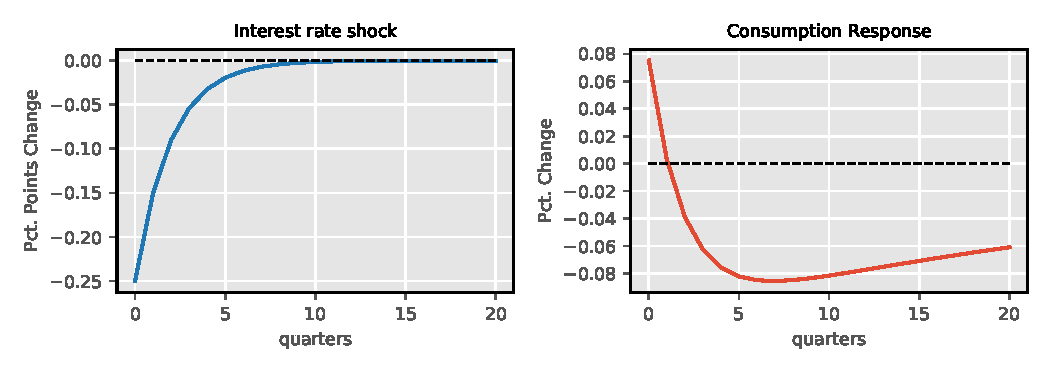
\includegraphics[width=.98\linewidth]{mainmatter/plots/SS_evaluation/Consumption_interest_rate_response.pdf} 
}
\caption{Impulses to a temporary interest rate shock analogues to \citet{kaplan2018monetary}.}
\label{fig:calibration_C_r}
    \scriptsize
    \centering
    {
    \emph{Note:} Response to a -0.25 percentage point drop in the real interest rate with persistence 0.6. }
 % {\scriptsize  Impulse responses to a negative productivity shock of 1\% with persistence 0.94 (half-life: 5 quarters). }
\end{figure}


\subsubsection{Liquid vs. Illiquid assets.} As an example of this compositional effect arising in the KV two-asset model, consider the following example: Imagine that assets $a_{i,t}$ is composed of 10\% liquid assets which yields return $r$ set by the central bank, and 90\% percent illiquid assets $\bar{a}_i$ which yields exogenous return $\bar{r}$, which equals the steady state return. Assume further that the Euler equation uses the rate $r$. Figure \ref{fig:dC_dR_illiquid_example} in the appendix shows consumption responses under this calibration. The response moves closer to the RA response, and closely resembles that from Kaplan et. al. Note though, that in the KV-model changes in the monetary policy rate also affects the return to illiquid assets and hence also generates changes to financial income. This, however, occurs only in the general equilibrium where the monetary policy rate affects the return to capital and firm equity. 

%no-arbitrage conditions between the return to liquid and illiquid assets imply that the return to illiquid assets are directly affected by interest rate changes. The crucial mechanism w.r.t the consumption response is that the presence of adjustment costs for illiquid assets ensures that this stock adjusts only slowly to 



These considerations tie directly into the discussion of whether the calibration of single asset macroeconomic models should reflect overall net worth or only liquid assets, see in particular \citet{carroll2017distribution}. Carrol et. al. show that their "Beta-dist" model - which closely resembles the household model in this paper - matches empirical MPCs well, and does so in a simpler setting than the KV two-asset model. However, as shown here the weakness of the "beta-dist" model is that it generates a relatively volatile consumption response to a real interest rate shock. The KV model, and by extension the two-asset HANK model, excels in this regard. 


\subsubsection{Borrowing} Note that allowing for borrowing (i.e. allowing $a_{i,t}<0$) aids the one-asset HANK model in replicating the interest rate response of the KV HANK model since a monetary policy loosening implies a decrease in interest payments on debt and hence an increase in income for indebted households.  However, allowing for borrowing up to usual amounts (one quarterly wage rate for unsecured borrowing, which borrowing is to be interpreted under my calibration) gives rise to an unrealistic wealth distribution where large parts of the population is indebted if there is no interest rate differential. 
%Allowing for different interest rates to debtors and creditors creates a borrowing wedge, which replicates realistic wealth distributions by generating large masses of household around the zero net-worth cutoff. The solution to the households problem is however complicated since there is a kink in the budget constraint at $a_{i,t} = 0$. As a consequence a more general EGM method, as discussed in \citet{druedahl2019guide}, must be applied. For this reason I calibrate the borrowing limit to match share of households in debt, with the resulting limit being less than the quarterly wage rate-limit usually assumed.   
%However, for realistic borrowing limits - usually considered to be one quarterly wage rate for unsecured borrowing - this mechanism is not sufficiently large to alleviate the issue.  
%This is of course a direct application of the unhedged interest exposure channel discussed above.

% Unheged interest exposure 
%\subsubsection{Debt Maturity.} Obviously the simplistic structure of households balance sheets matter for the interest rate response. As is common in simple NK models all assets of the household mature every period, and hence changes in the interest rate has full pass-through onto financial income. A more complete modeling of household balance sheets and asset compositions where maturity is not immediate will also provide more realistic responses. Debt maturity can be easily implemented in the governments supply of bonds (see \citet{auclert2020micro}), but it is less obvious to implement in firm equity since dividends are generated each period.  







\subsection{Dynamic Consumption Responses - Discount Factor Heterogeneity} \label{sec:C_robustness_disc}
To better explain consumption and welfare changes across households Figure \ref{fig:calibration_C_r_beta} considers the average consumption responses for each of the different discount factor groups in the baseline model. Through a close correlation with the wealth distribution (recall table \ref{table:Wealth_dist}), the model displays a wide amount of heterogeneity in responses by discount factors. For the income shock the contemporaneous (annual) MPC varies from 0.05 to roughly 0.6 with the min/max MPCs being represented by the lowest and highest discount factor groups respectively. Furthermore, the persistence of the income shock declines monotonously in discount factors. To this end, recal that in the  limiting case where households act as HtM agents exhibit zero persistence.    

For the interest rate shock the responses are also prone to heterogeneity. For patient households the on-impact effect of a lower interest rate is relatively low, and almost negative for the most patient households. The reason, as argued earlier, is that the drop in financial income generates a persistent consumption drop, and even though a drop in the relative price of consumption implies more consumption today the high marginal utility in the future due to lower income implies that consumption today must be cut. For impatient households, who hold less wealth, the financial income channel is weak and their response more closely resemble that of a representative agent where the on-impact effect is governed primarily by the drop in the relative price of consumption. Note also that for impatient households a larger share of households tend to be indebted and a drop in the interest rate hence reduces interest payments thus increasing consumption.  


%though this tendency is not strict. From the 2nd quarter and onwards consumption declines, with the decline being monotone in discount factors. This stems from the correlation between $\beta$ and wealth: The effect of a change in the interest rate in the budget constraint is $a_{i,t-1}dR_{t}$ and is hence proportional to the level of wealth, and patient households who have accumulated high levels of wealth are hence subject to large drops in financial income compared to less patient households. 


% ADD LIQUID VS ILLIQUID WEALTH SECTION 

\begin{figure}[H]
\centering
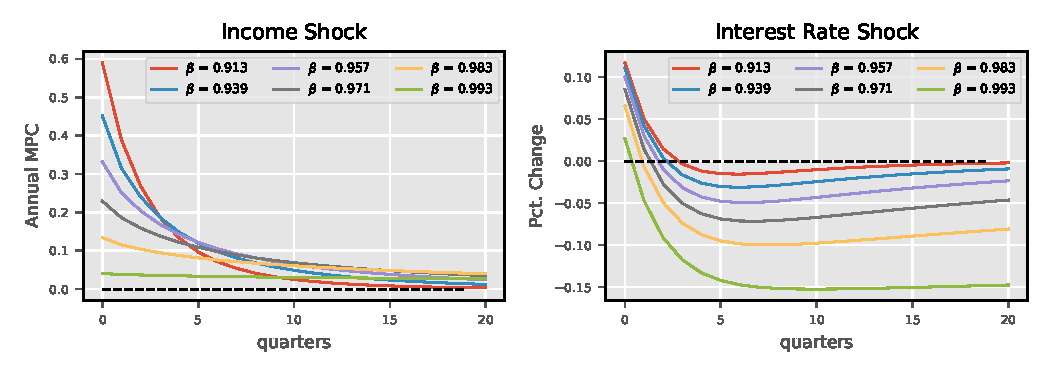
\includegraphics[width=.98\linewidth]{mainmatter/plots/SS_evaluation/Alternative_calibs/beta_dR_dI.pdf} 
\caption{Consumption responses to income and interest rate shocks by discount factor.}
\label{fig:calibration_C_r_beta}
\end{figure}


The appendix, section \ref{sec:C_robustness}, considers the consumption responses by different values of the standard deviation of earnings and the intertemporal elasticity of substitution, conditional on the wealth distribution. The standard deviation matters little when calibration to the wealth distribution, but the value of the intertemporal elasticity matters greatly. 



\subsection{Timing} 
As I analyze a persistent shock to the interest rate it involves both static effects as well as forward looking, exceptional effects. The static effect occurs in period 0 and involves no forward-looking behavior as the shock is unexpected, and consists only of a drop in financial income occurring through a lower interest rate. The forward-looking channel occurs both directly through changes to the future interest rate (since the shock is persistent, and the interest rate appearing in the Euler equations is that of the next period) as well as through changes to future marginal utilities of consumption. The second channel can potentially be strong in the general equilibrium, weak but persistent shock can be propagated since households precautionarily cut consumption today in expectation of having to smooth consumption over the duration of the shock.
I note once again that this is still a partial equilibrium setting, so even though the job-finding rate changes employment and wages stays constant. 
 

\begin{figure}[H]
\centering
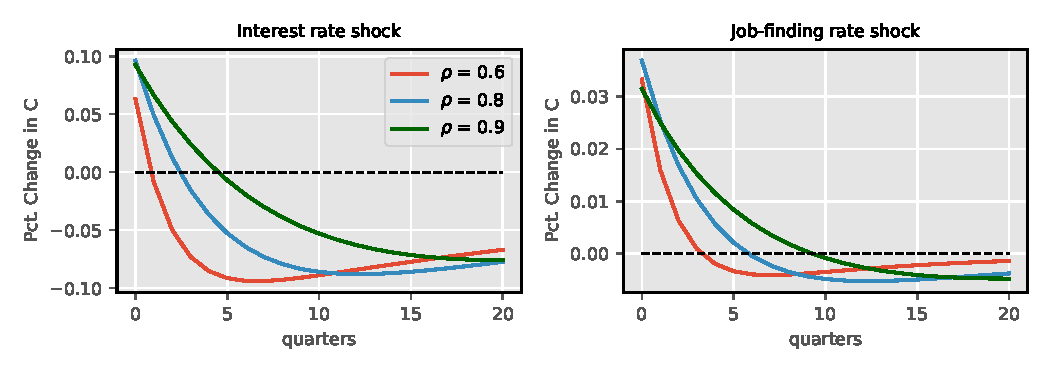
\includegraphics[width=.98\linewidth]{mainmatter/plots/C_analysis/ra_q_shocks_C.pdf} 
\label{fig:C_analysis_q_r}
\caption{Consumption responses to interest- and job-finding rate shocks with differing persistent.}
    \scriptsize
    \centering
    {
    \emph{Note:} Each panel plots the consumption response to a shock to either the real interest rate or the job-finding rate. The baseline shocks have $\rho=0.6$ with the -on-impact drop being 0.25 pct. points and 5\% for the two shocks respectively. The shocks with $\rho=0.8,0.9$ have been re-scaled such that the cumulative shock are the same across the shocks.   }
\end{figure} 

As the latter part of the thesis investigates persistent labor market dynamics, I here foreshadow this a bit in investing the effect of more persistent shocks to the job-finding rate. Figure \ref{fig:ra_q_shocks} in the appendix plots the shocks, Figure \ref{fig:C_analysis_q_r} plots the consumption responses. In interpreting the shocks there are two things to note. Since the Euler equations are forward looking in interest rates an unexpected change affects contemporaneous consumption only through changes in financial income, not intertemporal substitution. Similarly an unexpected change in the job-finding rate has no affect on consumption in period 0 \textit{when keeping employment fixed}, again due to the forward-looking nature of the Euler equations. Hence precautionary motives from unemployment risk are only induced when shocks to the finding rate are persistent and expected. 

The figure shows for both shocks that even though the most persistent shock is roughly 5 times as small on impact the effect on contemporaneous consumption is roughly the same across the shocks. Additionally and unsurprisingly, the more persistent shocks also generates more long-lived responses.  
As a side note, the shock to the job-finding rate shows that a persistent increase in-job finding rates increases only consumption by a marginal 0.03\%, with an on impact elasticity of $0.006$ for the least persistent shock. The most persistent shock has an elasticity of $0.03$.



%\subsubsection{Behavioral and distributional effects}
\subsection{Representative-Heterogeneous Agent Equivalence} \label{sec:Aggre_result} %  - An Aggregation Result
\subsubsection{Canonical Household models.} In the above discussion, I make numerous references to the canonical representative (or Ricardian) agent household structure, and the two agent model of \citet{campbell1989consumption}. The representative agent model is characterized by complete markets. The presence of these markets imply that households can perfectly insure against idiosyncratic and labor market risk, and essentially all risk that does not affect households equally.\footnote{More formally the assumption of complete markets assume the existence and availability of a complete set of Arrow-Debreu state contingency claims such that households can insure against every possible state. Trading these claims amongst themselves imply that all households obtain the same marginal utility of consumption, and are hence symmetric.} Appendix \ref{sec:RA_TA} contains the details, but optimization implies that consumption obeys the Euler equation:
\begin{gather*}
\left(C_{t}^{R}\right)^{-\frac{1}{\sigma}}=R_{t+1}\beta\left(C_{t+1}^{R}\right)^{-\frac{1}{\sigma}}
\end{gather*}
where $C^R$ denotes consumption of the representative/Ricardian/Rational agent. This results in a permanent-income setup where transitory income shocks have only marginal effects on current consumption. To counter this empirical oddity, \citet{campbell1989consumption} added Hand-to-Mouth households to the model, the resulting model being the two-agent (TA) model. HtM households holds no savings and consume their entire income each period, with resulting MPC equal to 1. Let $\lambda$ denote the share of HtM household. Consumption of these household is: 
\begin{gather*}
C_{t}^{HtM}=\left(\lambda I_{t}-\tau\left(\lambda I_{t}\right)+\lambda T_{t}\right),
\end{gather*}
with resulting aggregate consumption $C_{t}=C_{t}^{R}+C_{t}^{HtM}$. The share of HtM households $\lambda$ allows the model to capture two extreme states: For $\lambda=0$ shocks are very persistent since Ricardian households smooth consumption extensively, but MPCs are only marginal. For $\lambda=0$ the aggregate MPC is equal to 1 but shocks have no persistence. 
% proof \ref{Agg_result_proof}

% WTIHIN VS BETWEEN EFFECTS
% HANK = BETWEEN
% RANK/TANK = WITHIN 

%Keeping the distribution fixed imply that households are either always constraint or always obeying the Euler equation, and do not shift endogenously between these two states. This in turn that implies that   

\subsubsection{An Aggregation Result.} I now briefly compare the HA-household responses to the RA/TA-household responses in a partial equilibrium. Suppressing dependencies of the consumption function $c_{t}^{*}\left(a_{i,t},e_{i,t},\beta_{i},k_{i,t}\right)$ aggregate consumption is given by $C_{t}=\int c_{t}^{*}d\mathcal{D}_{t}$. A first-order perturbation around the steady-state yields: 
\begin{gather*}
dC_{t}= \underbrace{\int dc_{t}^{*}d\mathcal{D}_{ss} }_{\text{Static Effect}} + \underbrace{\int c_{ss}^{*}d\mathcal{D}_{t}}_{\text{Distributional Effect}} 
\end{gather*}
The firm term, which I dub the "static effect", captures how individual consumption changes \textit{conditional on placement in the earnings and asset distribution.} Since the placement in the ergodic distribution is determined by the dynamics of the budget constraint, the static effect - which holds constant this channel - corresponds to the dynamics of the RA (if no households are constrained in the steady-state) and TA models (if there exists constrained households in the steady-state): For rational, forward looking agents the Euler equation governs all dynamic responses, and for hand-to-mouth agents the budget constraint contains by definition no dynamics. Hence the difference between RA/TA and HA models in the partial equilibrium can be captured by the term $\int c_{ss}^{*}d\mathcal{D}_{t}$ to the first-order. Alternatively, the "static effect" term can be interpreted as a within-group effect and the "distributional effect" term a between-group effect. Appendix \ref{Agg_result_proof} contains a formal proof that the static effect term aggregates to a RA/TA setup.
%, keeping wages fixed.\footnote{Fixing wages imply no endogenous change in labor supply. This simplifies aggregation since otherwise an interaction between labor supply and heterogeneous earnings occur. } 

Figure \ref{fig:C_decomp_over_dist} shows this decomposition for the income and interest rate shock discussed in detail earlier. Perhaps unsurprisingly, but nonetheless interesting, it shows that changes in the income and wealth distribution of households accounts for the majority of persistence in the partial equilibrium impulses. For the income shock the persistence is generated by the fact that the model features low-wealth households who simultaneously have high MPCs and are forward looking. For the interest rate shock persistence is generated by a transitory drop in financial income. 


\begin{figure}[H]
\makebox[\linewidth][c]{%
\centering
  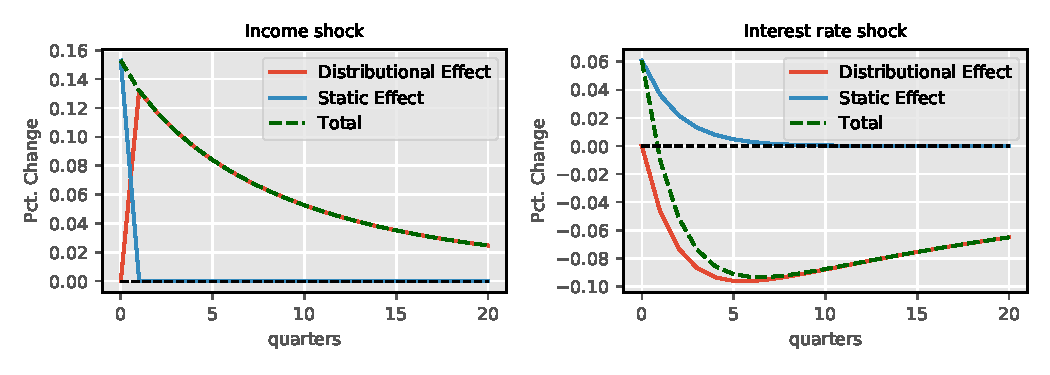
\includegraphics[width=.98\linewidth]{mainmatter/plots/C_analysis/dC__decomp_dist.pdf} 
}
\caption{HA responses decomposed in static and distributional effects. }
\label{fig:C_decomp_over_dist}
%\centering
 \scriptsize  
 \emph{Note:} The Static effect $\int dc_{t}^{*}d\mathcal{D}_{ss}$ in response to a shock keeps constant the distribution of households across states, while the distributional effect $\int c_{ss}^{*}d\mathcal{D}_{t}$ keeps constant consumption decisions. To a first-order approximation the total effect is the sum of the two effects. 
\end{figure}

\begin{figure}[h]
\makebox[\linewidth][c]{%
\centering
  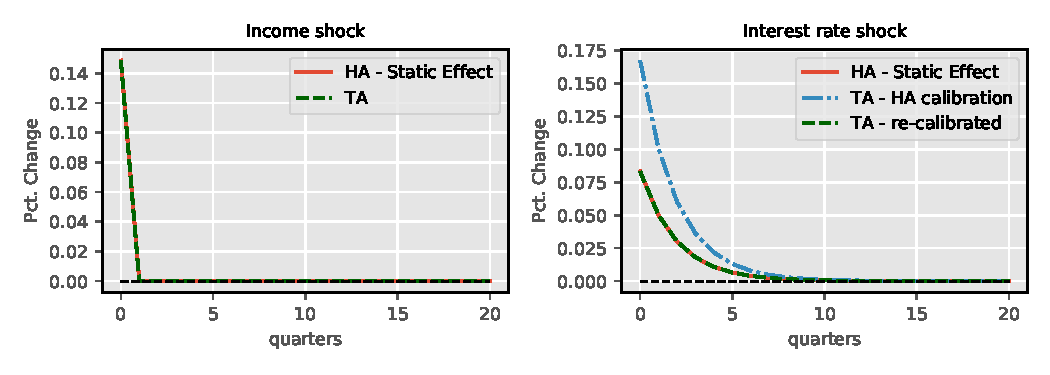
\includegraphics[width=.98\linewidth]{mainmatter/plots/C_analysis/TANK_vs_HANK_behavoiral_decomp.pdf} 
}
\caption{static from HA vs. TA responses.}
\label{fig:HANK_vs_TANK}
    \scriptsize
    {
    \emph{Note:} Each panel plots the static response $\int dc_{t}^{*}d\mathcal{D}_{ss}$ from the HA model against a calibrated TA. The TA model's share of HtM consumers is calibrated to match the initial MPC of the HA model. The 'TA - HA calibration' model refers to a TA-model with the interest rate from the HA model, while 'TA - re-calibrated' re-calibrates the interest rate and discount factor to match the initial response of consumption to an interest rate shock in the HA model.}
\end{figure}

Figure \ref{fig:HANK_vs_TANK} shows the extent of the equivalence. The left panel plots the static effect from the HA model $\int dc_{t}^{*}d\mathcal{D}_{ss}$ against a standard TANK model for the income shock, with the share of HtM consumers in the TA model calibrated to match the initial MPC of the HA model.\footnote{The RA/TA models are described in appendix \ref{sec:RA_TA}.} The two responses intersect exactly. \\
The right side panel conducts a similar exercise for the interest rate shock. However, here calibration matters to a larger extend. Applying the same interest rate as in the HANK model implies a discount factor of $\beta^{TA}=\frac{1}{1+r_{ss}^{HA}}-1$ in the TA model. Due to precautionary savings, this RA discount factor is significantly higher than the average discount factor in the HA model. This explains the majority of the difference between the HA and TA (HA calibration) responses in the panel. To this end, I re-calibrate the real interest rate in the TA model (and hence the discount factor) to match the initial response of the HA model. Again, the two curves intersect exactly. Thus the HA model contains the TA model as a special case where the term ${\int c_{ss}^{*}d\mathcal{D}_{t}}$ is held constant, \textit{conditional on calibration}.





\begin{figure}[h]
\makebox[\linewidth][c]{%
\centering
  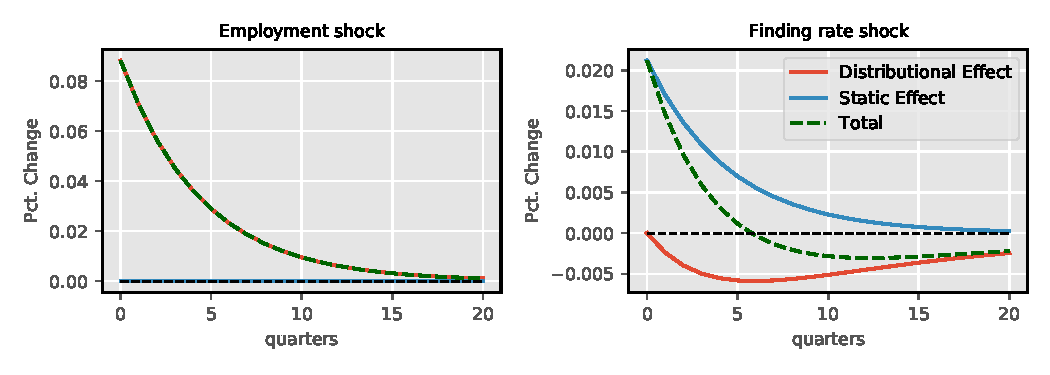
\includegraphics[width=.98\linewidth]{mainmatter/plots/C_analysis/dC__decomp_dist_N_q.pdf} 
}
\caption{HANK responses decomposed in static and distributional effects for a positive employment and job finding rate shock respectively. }
\label{fig:C_decomp_over_dist_N_q}
\centering
    \scriptsize
    {
    \emph{Note:} Each panel decomposes the total response to a shock in a distributional and a static response. The left panel considers a 1\% increase in employment with persistence 0.8, and the right panel considers a positive job-finding rate shock with the same proprieties.}
\end{figure}

\subsubsection{Employment and job-finding rates.}  Figure \ref{fig:HANK_vs_TANK} shows the distributional/static decomposition for a positive employment shock and a positive job-finding rate shock. The employment shock consists only of the distributional effect of shifting households from an unemployed state to an employed state since I keep the job-finding rate constant. The shock, however still delivers a more persist response than the underlying shock due to wealth accumulation. For the job-finding rate shock the static effect through the Euler equation dominates the total response, 
Note that the contemporaneous effect on consumption from higher employment equals exactly the average difference between consumption of employed and unemployed households in steady-state. \footnote{$dC_{t}=C_{ss}^{k=N}N_{t}-C_{ss}^{k=U}N_{t}\Leftrightarrow\frac{dC_{t}}{C_{ss}}=\frac{C_{ss}^{k=N}-C_{ss}^{k=U}}{C_{ss}}N_{t}$.} Due to households self-insuring against unemployment risk this consumption wedge is significantly less than the replacement ratio of 51\% (roughly 14\%), and the impact of employment changes is lessened. 


%\subsubsection{Heterogeneity, wealth accumulation and persistence.} Figure \ref{fig:HANK_vs_TANK} reveals that one significant dimension which the HA-model contributes to is persistence. Because shocks to income and interest rates move households around in the wealth distribution, and this in turn affect future consumption/savings decisions, these shocks have long lasting effect compared to the RA/TA-counterparts. To further exemplify this channel, consider figure \ref{fig:C_decomp_over_dist_N_q}, which decomposes the HA response to a positive employment shock and a positive job finding rate shock 
%\footnote{While the "behavioral" effect of the HA model has a direct equivalence to the TA household model when considering income and interest rate shocks, this is not necessarily the case for the job finding rate shock. If the TA household model derives from a  representative family construct, complete insurance imply changes in the finding rate has no affect on consumption, holding employment fixed. To obtain responses comparable with the HA model one needs to assume uninsurable unemployment risk.} 


%For instance, for the employment shock the behavioral effect (RA/TA-effect) has faded out after 20 quarters, whereas the distributional effect is still well above the steady-state level. 




%\subsection{Reflection} % Job finding rate response. 
%I have so far considered how consumption reacts to changes in disposable income and interest rates, which are the two primarily channels that may affect consumption. Consider for a moment how each of these channels are affected by the business cycle. 

% C makes up roughly half of Y in DK 
% more volatile than GDP, but 1/3 as volatile as I. However I share of Y is 16%. 


%In typical NK models changes in disposable income are generated by changes in wages, employment, lump sum transfers and, potentially, dividends. Wages are usually considered very rigid, almost acyclical, and dividends are modeled as firm equity, not transfers. Hence it is mostly employment and lump sum transfers that can move disposable income and hence consumption. As per the exposition above, interest rates affect consumption, but probably not enough to account for the aggregate volatility observed. What remains to affect consumption decisions is essentially precautionary savings, i.e. the fact that households increase savings by cutting consumption when faced with an increase in risk. In the present model the only source of cyclical risk is through the labor market job-finding rates. 


%The remaining channel affecting consumption is not related to income or financial flows but rather behavior and expectations. In
% Add section analyzing finding rates? 


\subsection{General Equilibrium Transmission of a TFP Shock}


%\subsubsection{Baseline Impulse Responses}
% Size of shock? 
%This section briefly dissects a negative investment shock in the baseline model (a shock to $Z^I_t$). I will use this type of shock as the main source of exogenous variation in the model, partly because it is the main driver of business cycles according to some (\citet{justiniano2010investment}), but also because this type of shock can generate labor and capital responses with same sign, which is not necessarily the case with a TFP shock. This simplifies the analysis. 
%also Corona crisis 

\subsubsection{Baseline Impulse Responses.}
I now move to the general equilibrium model described in detail in section \ref{chap:Model1}. For this purpose, I subject the model to an unanticipated, 1\% negative productivity shock with persistence 0.8. Since impulse responses are obtained through first-order approximations the responses are symmetric to the sign of the shock, and all considerations apply equally to a positive shock. Figure \ref{fig:baseline_impulse} shows the results. 
%In this experiment the government adjusts only bonds taxes to satisfy its budget constraint. Under different circumstances, this would accompanied by a tax reaction function which ensures that public debt does not explode, but given the shape of the shock and stability of the remaining model blocks, government debt converges back to the steady-state level even without changes in taxation. Thus I simplify the analysis by simply omitting the tax reaction function.  

The unexpected decrease in productivity increases the real marginal costs of firms, and hence prices. However, due to Keynesian frictions (nominal rigidities) prices only take some of the adjustment, and employment and investment hence decline due to lower marginal products. Lower employment and wages implies a drop in aggregate demand. Furthermore, consumption also declines for precautionary reasons as the job-finding rate drop. The central bank responds to the increase in inflation by increasing the real interest rate through the nominal rate. This is consistent with empirical evidence for neutral technology shocks, see for instance \citet{christiano2016unemployment}. 
%, leading to a partial stabilizing of demand in the contemporaneous period, but prolonging the negative effects of the shock.\footnote{Note that investments tends to overshoot in response to a negative shock. This comes from particular functional form of investment adjustment costs.} 

The middle panel of the figure displays the response asset variables (Households assets $A$, government bonds $B$ and firm equity $p^e$). In response to the negative shock government revenue from income and consumption taxes decline and expenses to unemployment benefits increases, 
and to maintain budget balance more bonds are issued. 
%To avoid explosive debt dynamics this turn forces the government to cut transfers to households, albeit with a lag.  
For firms the economic downturn imply a decrease in profits and dividends. Since firm equity equals the discounted stream of future dividends the value of firm shares drop. Overall, household's stock of wealth increases from period 1 and onwards. Compared to models which features only firm equity and/or capital as assets Keynes' paradox of thrift is partially alleviated here since the government issues debt over the cycle to fill the gap from lower tax revenue, thus acting as a buffer for household savings. In models with only capital/firm equity the paradox of thrift implies that household savings increase in the partial equilibrium for precautionary reasons but decrease in the general equilibrium since the drop consumption decreases demand and hence firm profits/dividends and capital, leading to a drop in the aggregate stock of assets. 


%\footnote{Simple NK models usually contain counter-cyclical markups such that profits/dividends increase in response to negative shocks. This is also the case in present model. }


%Since obviously the asset market is an important determinant of the dynamic response of the model, I will also discuss this a bit. The market equilibrium condition states that $A=B p^G + p^e$, i.e. household wealth equals the sum of government bonds and firm equity. Each component in this balance is affected wildly different by the shock. 
%For household wealth there are opposing forces: Aggregate income drops, and the real interest declines - this speaks to a decline in assets. However, as the job finding rate declines households increase savings for precautionary reasons, which speaks to an increase. 

%I consider a relatively persistent shock to technology since otherwise the initial positive effect on employment dominates, and the adverse effects from declining job finding rates are non-existent. The fact that an adverse technology shock initially stimulates employment (and vice-versa for a positive shock) is common in medium scale DSGE models - see for instance the impulses in \citet{pedersen2013drives}, \citet{christiano2016unemployment} etc. 

Overall, the shock is consistent with magnitudes in \citet{gornemann2016doves}, though the shock presented here contains significantly more persistence, mainly due to the dynamics of public debt, something which is entirely left out in \citet{gornemann2016doves}.\footnote{Gornemann et al. assumes no public debt, and that a proportional tax on labor income is adjusted at every instant to finance unemployment benefits.}

%The employment response (and consequently the job-finding rate) is rather volatile, though this is not totally unwarranted. \citet{christiano2016unemployment} estimates a peak response of output of 0.4\% following a one standard deviation TFP shock. The response of employment is 0.1\% and for the job-finding rate 1\%. The implied elasticities w.r.t output are 0.25 and 2.5 respectively. The comparable elasticities in my model are 0.94 and 5.   

%Note though that there model features utilization. This implies that labor and capital quantities need to move less to obtain a given output response. 

\begin{figure}[H]
\makebox[\linewidth][c]{%
\centering
  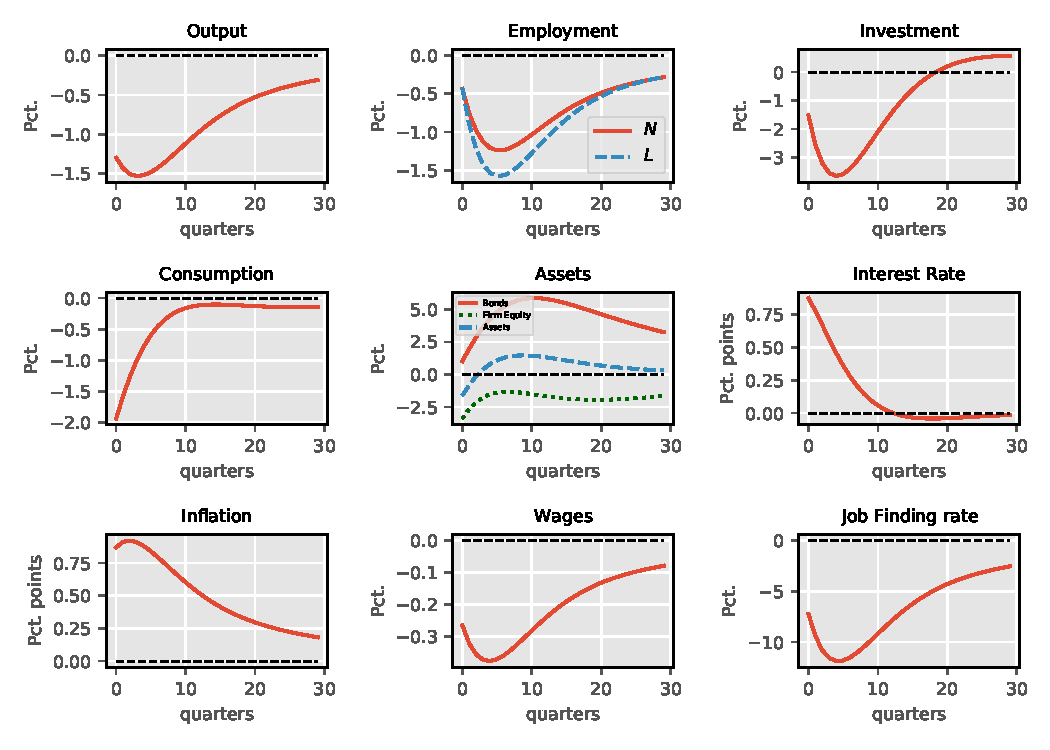
\includegraphics[width=.98\linewidth]{mainmatter/plots/SS_evaluation/main_shock.pdf} 
}
\caption[Caption for LOF]{Impulse responses to a negative productivity shock.}
\label{fig:baseline_impulse}
\scriptsize
\centering
\emph{Note:} Impulse responses to a negative productivity shock of 1\% with persistence 0.8. 
\end{figure}

%\begin{figure}[H]
%\makebox[\linewidth][c]{%
%\centering
%  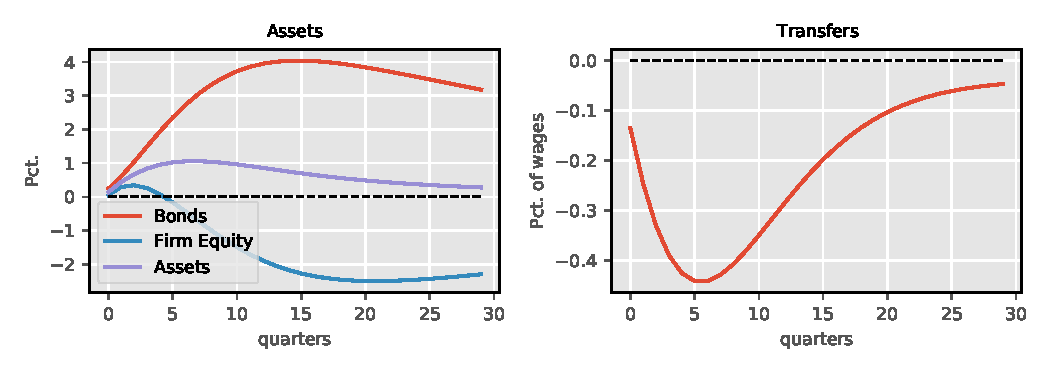
\includegraphics[width=.98\linewidth]{mainmatter/plots/SS_evaluation/Assets_transfers.pdf} 
%}
%\caption[Caption for LOF]{Responses of assets and transfers.}
%\label{fig:baseline_impulse_assets_transfers}
% % {\scriptsize  Impulse responses to a negative productivity shock of 1\% with persistence 0.8. }
%\end{figure}
\subsubsection{Decomposing Aggregate Consumption.}
Aggregate consumption $C_{t}$ is a function of paths $\left\{w_{t},r_{t},q_{t},N_{t}\right\} _{t\geq0}$, and given a particular general equilibrium path $\left\{ x_{t}\right\} _{t\geq0}\in\left\{w_{t},r_{t},q_{t},N_{t}\right\} _{t\geq0}$ the effect of this particular $x$ on $C$ can be obtained by a first-order approximation. Figure \ref{fig:baseline_C_decomp} shows the resulting decomposition. Half of the initial drop is caused by higher interest rates, while increased unemployment risk through lower job-finding rates account for 1/3 of the drop. Lower wages and higher unemployment account for the remaining drop. The majority of the consumption response can be said to be driven by the interest rate, though the job-finding rates has a non-trivial effect too. 

\begin{figure}[H]
\makebox[\linewidth][c]{%
\centering
  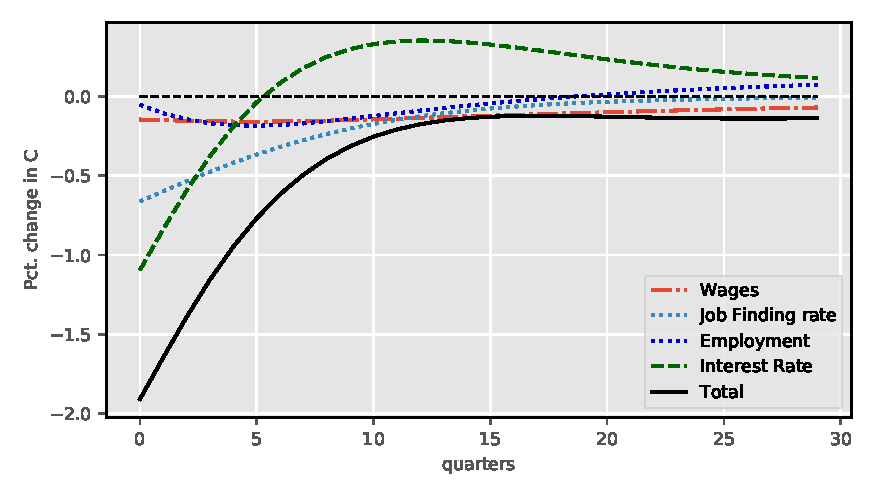
\includegraphics[width=.6\linewidth]{mainmatter/plots/SS_evaluation/C_decomp_main_G.pdf} 
}
\caption[Caption for LOF]{Decomposition of Consumption in response to a negative productivity shock. }
\label{fig:baseline_C_decomp}
\centering
\scriptsize
\centering
\emph{Note:} Decomposed responses sum to total.
\end{figure}

%Lump-sum transfers account for the majority of consumption response. This observations is common to HANK models. In \citet{kaplan2018monetary} public transfers account for roughly 1/3 of the consumption response resulting from a monetary policy shock. \\
%Half of the initial drop in consumption comes from a drop in the job finding rate through precautionary motives. The persistent drop in consumption in the following periods is driven by lower income to the household sector through different channels. 1) The government reduces transfers to satisfy debt obligations, 2) The drop in interest rates reduces financial income, and 3) A persistent drop in employment implies that more households must make due with public benefits which are roughly half of the wage rate. 


\subsection{Heterogeneity In Consumption Responses } % - Welfare Implications.
Before evaluating the welfare implications of the shock I consider the disaggregated consumption response. The left panel of Figure \ref{fig:baseline_C_decomp_disagg} displays the on-impact drop in consumption following the TFP shock by wealth deciles, along with a decomposition which serves to identify the drivers of consumption across the wealth distribution. The relative drops in consumption are monotone across wealth deciles, with the poorest households exhibiting the largest consumption drops. 
The decomposition reveals that the mechanisms behind are not entirely homogeneous. For the poorest wealth decile the largest contributing factor is higher unemployment risk, which induces precautionary savings. This channel is particularly strong for the poorest households since these are weakly insured against adverse shocks. Higher interest rates also accounts for a significant part of the decline, partly due to intertemporal substitution but also due to an increase in interest payments on debt.\footnote{Recall from the calibration that the entire 1st wealth decile are in debt.} 
As one moves up the wealth deciles the effect of increasing unemployment risk affects consumption less because households are better insured, and the defining factor becomes movements in the interest rates. 
For the wealthiest households changes in unemployment risk and wages matters very little because their asset holdings are so large that marginal utilities across employment states are always equalized. Accordingly, they almost only react to changes in the marginal rate of substitution between present and future consumption.  

%For the poorest wealth decile a large share is constrained from borrowing, and the effect of hike in the interest rate is hence lessened. Instead, the drop in the finding rate accounts for a large share of the drop in consumption for this class of workers. Since these households are poorly insured due to low savings they fear going into unemployment/staying unemployed for a longer duration more than wealthier households and the precautionary savings effect from higher labor market risk is significant. For wealthier households the higher interest rate imply that they postpone consumption, and this accounts for between 1/2-2/3 of consumption declines, with the finding rate being the second most important determinant. As shown in the consumption decomposition in figure \ref{fig:baseline_C_decomp} these considerations primarily apply to the first-period consumption response, since the drop in employment becomes more important w.r.t persistence than the finding rate. 

While the left panel of Figure \ref{fig:baseline_C_decomp_disagg} might lead one to think that stabilizing consumption is roughly equivalent with stabilizing consumption of households in bottom tail of the wealth distribution, the right panel shows that this is not necessarily the case.\footnote{When discussion stabilization in terms of stimulus to groups with high MPCs these consideration of course do not apply since MPCs are an absolute quantity, not a relative.} The change in aggregate consumption $dC_t$ can be written as an additive decomposition across wealth deciles, where each decile's contribution to the aggregate is given by $\frac{C_{i,ss}}{C_{ss}}\frac{dC_{i,t}}{C_{i,ss}}$. That is, the product of a static share $\frac{C_{i,ss}}{C_{ss}}$ (share of aggregate steady-state consumption of wealth decile $i$) and the relative change in the decile's consumption $\frac{dC_{i,t}}{C_{i,ss}}$ following the shock.\footnote{$dC_{t}=\sum_{i}dC_{i,t}\Leftrightarrow\frac{dC_{t}}{C_{ss}}=\sum_{i}\frac{1}{C_{ss}}dC_{i,t}=\sum_{i}\frac{C_{i,ss}}{C_{ss}}\frac{dC_{i,t}}{C_{i,ss}}$.} The left panel show the share of the aggregate consumption response in period 0 that each decile accounts for. This is the product of the left panel and the steady-state consumption shares (see appendix Figure \ref{fig:C_dist_by_deciles} for the steady-state distribution of consumption by wealth deciles). %Despite only accounting for 4\% of consumption the poorest households account for 15\% of the drop in aggregate consumption. For the remaining deciles the they each account for roughly an equal share. 
Despite having a consumption drop of almost 5\% the poorest decile - over double the aggregate drop of 2\% - these households have a less-than proportional affect on aggregate consumption, accounting for only 9\% of the drop. Instead the households in the lower-middle of the wealth distribution account for more than their weight, while the top decile has only a small effect on aggregate consumption. 
% More here 



%The fact that a major part of the transmission mechanism acts through transfers is not uncommon in HANK models, and is further amplified when rigid wages are present. A large part of the recent literature ignores this since wages are relatively flexible and thus accounts for a large share of the consumption response. This is for instance the case in \citet{auclert2020micro} who discusses a propagation mechanism where higher investment increases wages by increases the marginal product, thus in turn increasing consumption and output due to the high MPCs present in HANK models. 

%The reason for this relatively straightforward: While a decrease in wages hurts the government budget balance through lower income taxes, the impact is even greater when households move from employment to unemployment. Hence, when wages are more flexible and employment moves less over the cycle a smaller reduction in transfers is needed to satisfy the government budget constraint and wages thus substitute for transfers in a way. 



\begin{figure}[H]
\makebox[\linewidth][c]{%
\centering
  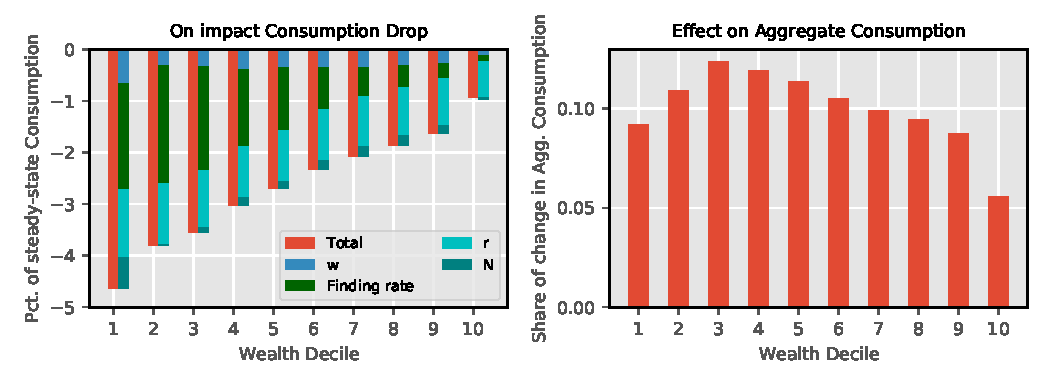
\includegraphics[width=.95\linewidth]{mainmatter/plots/SS_evaluation/peak_c_by_decile.pdf} 
}
\caption[Caption for LOF]{Decomposition of Consumption by Wealth Deciles. }
\label{fig:baseline_C_decomp_disagg}
\centering
\scriptsize 
\emph{Note:} The decomposed column might not add to the total due to first-order approximation errors.  
\end{figure}


\footnote{I first calculate the aggregate wealth deciles in the entire population. Afterwards, I divide households by employment status within each wealth decile. }


I follow \citet{gornemann2016doves} in evaluating the welfare implications of shocks. They compute lifetime consumption equivalent welfare gains/losses, defined as the amount of consumption that a given household is willing to give up to experience a certain event, here a persistent, negative TFP shock.\footnote{Let $U_{t_{0}}^{k}\left(\left\{ c_{i,t},\ell_{i,t}\right\} _{t=t_{0}}^{^{T}}\right)=\int\sum_{t=t_{0}}^{T}\beta_{i}^{t}u\left(c_{i,t},\ell_{i,t}\right)d\mathcal{D}_{t,k}$ denote discounted welfare for some group of households $k$ (percentiles, quantiles, employed, unemployed etc.) from time $t_0$ to $T$. The lifetime consumption equivalent of this group in response to the shock solves $U_{ss}^{k}\left(\left\{ \left(1+x\right)c_{i,ss},\ell_{i,ss}\right\} \right)=U_{t_{0}}^{k}\left(\left\{ c_{i,t},\ell_{i,t}\right\} _{t=t_{0}}^{^{T}}\right)$ for $x$. I use a horizon of 300 quarters, with $t_0$ being the impact period of the shock.  }
Figure \ref{fig:C_equiv_Baseline} displays the lifetime Consumption-equivalent welfare loss following the TFP shock for three different household characteristics. The left and right panel displays the losses for employed vs. unemployed households respectively. Within each panel (and employment group) I consider the welfare loss by wealth deciles, and within each wealth decile, by skill type. The skill types are the 30th, 50th, and 70th deciles in the income distribution respectively.\footnote{Note that compared to \citet{gornemann2016doves} the welfare losses do not seem to be monotone in earnings percentiles. The reason is that their figures condition on discount factors, whereas mine do not.} 

Employed households are on average willing to trade off 0.5\% of steady-state consumption to avoid the shock, while unemployed on average are willing to pay to experience the shock, though this is driven strongly by the upper wealth deciles. The main reason for this is that the shock brings about higher interest rates which households in the upper deciles benefit greatly from due to increases in financial income. For households in the bottom and lower-middle in the wealth distribution lower wages and higher unemployment risk dominates this financial income channel and they experience a welfare loss following the shock. 
There is a significant difference between the welfare implications of employed and unemployed households. For employed households only the wealthiest decile benefit from the shock, whereas for the unemployed households the 7th-9th decile also benefits from the shock. [Discuss: wages?]

% why significantly different from gorneman et al? 

%As in Gornemann et. al. I find that the welfare losses are U-shaped in wealth. That is, the largest welfare losses occur not at the bottom or top of the distribution but in the middle. The 2nd decile suffers a larger welfare drop compared to the 1st decile due to precautionary savings: Within the poorest decile a large share is constrained, and only respond to changes in income. When moving up to the second decile less households are constrained, and they respond more to drops in the job finding rate. Furthermore, they tend to be more patient (higher $\beta$)and hence "suffer" more due to the persistence of the shock, contrary to very impatient households where only drops in consumption close to $t_0$ matters.  

Recall that unemployment benefits are only proportional to idiosyncratic earnings risk, but not the aggregate wage rate $w_t$.\footnote{In practice unemployment befits are indexed to wage growth, but usually with a lag. In Denmark this occurs through the \textit{satsregulering}, where public transfers are indexed to wage growth with a two year lag.} Hence unemployed households are not subject to any income drops other than through idiosyncratic risk. 


\begin{figure}[H]
\makebox[\linewidth][c]{%
\centering
  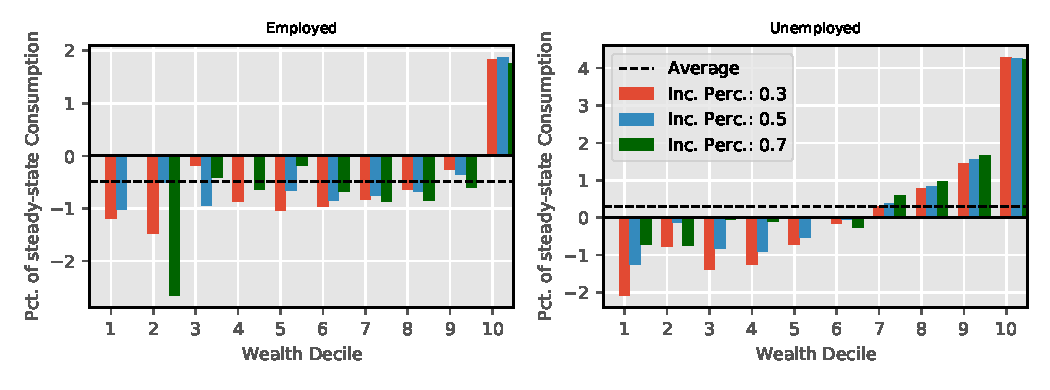
\includegraphics[width=.95\linewidth]{mainmatter/plots/SS_evaluation/C_equiv_by_e_N.pdf} 
}
\caption[Caption for LOF]{Consumption-equivalent welfare Loss by Type}
\label{fig:C_equiv_Baseline}
\centering

 % {\scriptsize  Note that the decomposed column might not add to the total due to first-order approximation errors. (Earnings percentile, employment status and wealth decile) }
\end{figure}


\subsubsection{Aggregate Inequality.} Figure \ref{fig:Inequality_response} (appendix) spells out the effects on aggregate inequality following the shock. Overall wealth and income inequality declines, but surprisingly consumption inequality increases. It is, however, notable that the share of wealth held by the top 5\% increases, and by a significant amount (0.4 percentage points at the peak). This is mainly due to the rise in interest rates since this group holds a disproportionately large share of aggregate wealth.     




%\subsubsection{Income Risk.}
%A heavily discussed feature of HANK models is income risk, and the cyclical element of it. Some papers assume acyclical risk (\citet{kaplan2018monetary}, \citet{hagedorn2019fiscal}), while others use ad-hoc, reduced form rules to model counter-cyclical risk \citet{acharya2020understanding}, \citet{auclert2018inequality}
%Pro-cyclical risk is usually not considered. My model features two separate sources of income risk: An exogenous and an endogenous channel. The exogenous channel is the earnings risk $e_i,t$ which directly affects household labor income. This gives rise to precautionary savings, but is constant over the cycle (acyclical). The endogenous channel is unemployment risk. In the presence of a search-and-matching labor market involuntary unemployment arises due to labor market frictions. In the baseline model households loose their job at an exogenous rate $\delta^L$, and re-obtain jobs at the endogenous job-finding rate $q_t$. Since the job-finding rate is counter-cyclical to the most common shocks this unemployment risk is countercyclical. The implication is that households increase savings if the job finding rate declines, and demand hence declines. This channel is extensively covered in \citet{ravn2016macroeconomic}.   



% r, Ravn and Sterk (2017), Werning (2015), Heathcote and Perri (2018), Beaudry, Galizia
%and Portier (2018), Kekre (2018), Bayer et al. (2019), Bilbiie (2019), and Acharya and Dogra (2019)